% Chapter Template
\newcommand{\drawkey}[3]{
    \draw[line width=0.07cm, draw=#2] (#1) circle [radius=0.15cm];
    \draw[line width=0.07cm, draw=#2] (#1 -0.15) -- ++(0,-0.4);
    \draw[line width=0.07cm, draw=#2] (#1 -0.35) -- ++(-0.2,0);
    \draw[line width=0.07cm, draw=#2] (#1 -0.51) -- ++(-0.2,0);
    \node[below, text=#2] at (#1 -0.6) {#3}
}

% Definizione del comando per disegnare la parentesi
\newcommand{\drawcurlybrace}[3]{% posizione finale, posizione iniziale, testo sopra
    \draw [decorate,decoration={brace,amplitude=10pt,mirror},xshift=-4pt,yshift=0pt]
    (#1) -- (#2) node [black,midway,xshift=-2cm] {};
}

\chapter{Fondamenti di Comunicazioni Sicure}
\label{Capitolo 2} 
\textit{In questo capitolo esamineremo le problematiche relative alla
    sicurezza nelle comunicazioni. Inizieremo con un'analisi degli
    strumenti matematici fondamentali che sono alla base della protezione dei dati,
    esplorando le tecniche crittografiche e i loro principi teorici. Successivamente,
    ci concentreremo su come queste tecniche vengono effettivamente applicate per
    garantire la sicurezza nelle comunicazioni sulle reti di computer.
    }
\section{Teoria}

Dalla crittografia classica, come il cifrario di
Cesare, fino alle tecniche più sofisticate del
ventesimo secolo, come i sistemi di cifratura a chiave pubblica, la storia della
crittografia è caratterizzata da una continua evoluzione e innovazione.
Le fondamenta sui cui si basa non sono cambiate, andiamo a vedere strumenti matematici che ne fanno parte.

\subsection{Hash Function}

Una funzione \textbf{hash crittografiche} è una funzione matematica che prende in input un messaggio di lunghezza arbitraria e restituisce un output di
lunghezza fissa, noto come digest.

\begin{equation}
    H: \{0,1\}^*  \to \{0,1\}^n
\end{equation}

\begin{itemize}
    \item $\{0,1\}^*$: rappresenta l'insieme di tutte le stringhe binarie di lunghezza arbitraria.
    \item $\{0,1\}^n$: rappresenta l'insieme delle stringhe binarie di lunghezza fissa $n$.
\end{itemize}

% Grafico per la funzione di Hash
\begin{comment}
\begin{figure}[h!]
    \centering
    \begin{tikzpicture}[scale=1.5, every node/.style={scale=1}]
    
    % Input message 
    \node[draw, minimum width=3cm, minimum height=1cm, align=center] (input) {Messaggio \\ $m \in \{0,1\}^*$};
    % Hash function box 
    %\filldraw[draw=black, fill=blue!30, rotate=270] (4,0) -- (6,0) -- (5.5,1) -- (4.5,1) -- cycle; 
    \node[draw, minimum width=3cm, minimum height=1cm, align=center, right=2cm of input] (hash) {Funzione di Hash \\ $H$};
    % Digest (output) 
    \node[draw, minimum width=3cm, minimum height=1cm, align=center, right=2cm of hash] (output) {Digest \\  $H(m) \in \{0,1\}^n$};
    % Arrows 
    \draw[->, thick] (input) -- (hash) node[midway, above] {Input};
    \draw[->, thick] (hash) -- (output) node[midway, above] {Output};
    
    % Labels for security properties 
    \end{tikzpicture}
\end{figure}
\end{comment}

\vspace{0.2cm}
\noindent
Le funzioni di hash crittografiche sono strumenti fondamentali nel campo della
sicurezza informatica, progettate per garantire l'integrità e l'autenticità dei
dati. Per questo motivo, a questo tipo di funzioni sono richieste le seguenti proprietà: 
\begin{itemize}
    \item \textbf{Resistenza alle collisioni}: devono essere progettate in modo tale che sia \\computazionalmente impraticabile invertire il processo, ovvero,  dato il digest è dificile risalire 
    al messaggio che lo ha prodotto.
    \item \textbf{Proprietà di diffusione}: una leggere variazione dell'input deve produrre un hash completamente diverso, questa è fondamentale per garantire che gli attaccanti non possano prevedere o
    manipolare il valore di hash a seguito di modifiche all'input.
\end{itemize}    

\begin{center}
    Aggiungere grafico sulle one way funcion
\end{center}

\subsection{Schemi crittografici}
Uno schema di cifratura è un insieme di algoritmi e funzioni che definisce come trasformare un messaggio in chiaro (plaintext) in un messaggio cifrato (ciphertext) e viceversa, al fine di garantire la confidenzialità e la sicurezza delle comunicazioni.
Formalmente possiamo rappresentarlo come una quintupla: 

\begin{center}
    \((\mathcal{P}, \mathcal{C}, \mathcal{K}, E, D)\)
\end{center}

\begin{itemize}
    \item \(\mathcal{P}\): Insieme dei messaggi in chiaro (plaintext).
    \item \(\mathcal{C}\): Insieme dei messaggi cifrati (ciphertext).
    \item \(\mathcal{K}\): Insieme delle chiavi utilizzate per la cifratura e decifratura, \textit{key space}.
    \item \(E: \mathcal{K} \times \mathcal{P} \to \mathcal{C}\): Funzione di cifratura.
    \item \(D: \mathcal{K} \times \mathcal{C} \to \mathcal{P}\): Funzione di decifratura.
\end{itemize}

\noindent
Deve esistere una relazione inversa tra le operazioni di cifratura e decifratura:
\begin{equation}
D(k, E(k, m)) = m \quad \forall m \in \mathcal{P}, \, k \in \mathcal{K}
\end{equation}
\noindent
Lo schema in \textit{Fig. \ref{fig:schema}}, mostra il funzionamento generale di uno schema crittografico. 
Tuttavia andando a caratterizzare le chiavi utilizzate nelle operazioni di cifratura e decifratura possiamo dare una prima classificazione:
\begin{itemize}
    \item se $K_1 = K_2$ allora si parla di un schema di crittografia \textit{simmetrico}.
    \item se $K_1 \neq K_2$ allora si parla di schema di crittografia \textit{asimmetrico}.
\end{itemize}

\begin{figure}[h!]
    \centering
    \begin{tikzpicture}[scale=1.5, every node/.style={scale=1}] 
    % Plaintext
    \node[draw, minimum width=3cm, minimum height=1cm, align=center] (plaintext) {Plaintext\\ $m \in M$};
    % Encryption box 
    \node[draw, minimum width=3cm, minimum height=1cm, below=1cm of plaintext, align=center] (enc) {Cifratura \\ $C = E(K_1,m)$};
    % Ciphertext 
    % se si riesce aggiungere delle linee di delimitazione che facciano intendere che in quesot modo il messaggio è protetto
    \node[draw, minimum width=3cm, minimum height=1cm, right=2cm of enc, align=center] (ciphertext) {Chiphertext\\ $c \in C$};
    % Decryption box 
    \node[draw, minimum width=3cm, minimum height=1cm, right=2cm of ciphertext, align=center] (dec) {Decifratura \\ $M = D(K_2,c)$};
    % Recovered message 
    \node[draw, minimum width=3cm, minimum height=1cm, above=1cm of dec, align=center] (plaintext2) {Plaintext\\ $m \in M$};
    
    % Arrows connecting the elements 
    \draw[->, thick] (plaintext) -- (enc) node[midway, above] {}; 
    \draw[->, thick] (enc) -- (ciphertext) node[midway, above] {}; 
    \draw[->, thick] (ciphertext) -- (dec) node[midway, above] {}; 
    \draw[->, thick] (dec) -- (plaintext2) node[midway, above] {};
    
    % Keys used for encryption and decryption 
    \drawkey{0,-2.1}{black}{$K_1$};
    \drawkey{6.8,-2.1}{black}{$K_2$};
    \end{tikzpicture}
    \caption{Funzionamento di uno schema crittografico}
    \label{fig:schema}
\end{figure}

\subsubsection{Simmetrici}

Come descritto precedentemente, in uno schema simmetrico si utilizza la stessa
chiave sia per le operazioni di cifratura che di decifratura. Ciò implica che le
due parti coinvolte nella comunicazione debbano possedere la medesima chiave
segreta, nota anche come chiave pre-condivisa (PSK - Pre-Shared Key). \\Questa
caratteristica fondamentale rende gli schemi di crittografia simmetrica\\
particolarmente veloci ed efficienti, esempi ne sono AES e DES.

\newpage

\noindent
Le loro caratteristiche li rendono ideali per:

\begin{itemize}
    \item \textit{Cifratura} di Dati: proteggere file e database memorizzati
    su disco, garantendo che le informazioni sensibili rimangano riservate anche
    in caso di accesso non autorizzato. Sia proteggere i dati mentre vengono trasmessi su reti.
    \item \textit{HMAC} (Hash-based Message Authentication Code): combinati
    con funzioni di hash, gli algoritmi simmetrici possono generare codici HMAC,
    che forniscono autenticità e integrità ai messaggi. Fondamentale per
    garantire che i dati non vengano manomessi durante la trasmissione.
\end{itemize}




\subsubsection{Asimmetrici}

In uno schema di cifratura asimmetrica, detto anche a \textbf{chiave pubblica}, lo spazio delle chiavi \(\mathcal{K}\) è costituito da una coppia di chiavi \((k_{\text{pub}}, k_{\text{priv}})\), dove:

\begin{itemize}
    \item La chiave pubblica \(k_{\text{pub}}\) viene condivisa liberamente e utilizzata da chiunque per cifrare
    messaggi destinati al proprietario della chiave.
    \item La chiave privata \(k_{\text{priv}}\) è mantenuta segreta dal
    proprietario e viene utilizzata per decifrare i messaggi cifrati con la
    corrispondente chiave pubblica.
\end{itemize}

\noindent
Quindi le due funzioni si riscrivono come:
\begin{equation}
    E: \mathcal{K}_{\text{pub}} \times \mathcal{P} \to \mathcal{C}
\end{equation}
\begin{equation}
    D: \mathcal{K}_{\text{priv}} \times \mathcal{C} \to \mathcal{P}
\end{equation}
\noindent
Le due chiavi sono matematicamente legate, ma è computazionalmente difficile \\ ottenere la chiave privata a partire da quella pubblica. Il funzionamento 
si basa sul concetto di \textbf{trapdoor} che rende possibile una funzione (come la cifratura o la decifratura) semplice per chi conosce un segreto (la chiave privata) ma estremamente difficile per chi non lo conosce.
\\

\noindent
Uno dei principali utilizzi della crittografia asimmetrica è il \textbf{Key-Exchange}, il quale consente di scambiarsi un'informazione segreta su un canale pubblico. La procedura
più conosciuta è quella proposta da \textit{Diffie-Hellman} ed è mostrata in \textit{Fig. \ref{fig:dh}}

\begin{figure}[h!]
    \centering
    \begin{tikzpicture}
        % Public parameter:
        \node[draw=none,fill=none,align=center] (public) at (0,1) {Public parameter: g, p};
        
        % Alice
        \node[draw] (Alice) at (-2,0) {Alice}; 
        \draw[thick] (Alice) -- ++(0, -4);
          
        % Calculations of Alice
        \node[draw=none,fill=none,anchor=east] (asecret) at ($(Alice) + (0,-1)$) {$a \in_{R} \{2,\dots,p-2\}$};
        \node[draw=none,fill=none,anchor=east] (Apublic) at ($(Alice) + (0,-2)$) {$A = g^{a} \bmod{p}$};
        \node[draw=none,fill=none,anchor=east] (akey) at ($(Alice) + (0,-4)$) {$K = (B)^{a} = g^{ba}$};
          
        % Bob
        \node[draw] (Bob) at (2,0) {Bob}; 
        \draw[thick] (Bob) -- ++(0, -4);
         
        % Calculations of Bob
        \node[draw=none,fill=none,anchor=west] (bsecret) at ($(Bob) + (0,-1)$) {$b \in_{R} \{2,\dots,p-2\}$};
        \node[draw=none,fill=none,anchor=west] (Bpublic) at ($(Bob) + (0,-2)$) {$B = g^{b} \bmod{p}$};
        \node[draw=none,fill=none,anchor=west] (bkey) at ($(Bob) + (0,-4)$) {$K = (A)^{b} = g^{ab}$};
         
        % Messages
        \draw[->,thick] ($(Alice)+(0,-2)$) -- ($(Bob)+(0,-2.5)$) node [pos=0.5,above,font=\footnotesize] {A};
        \draw[->,thick] ($(Bob)+(0,-3)$) -- ($(Alice)+(0,-3.5)$) node [pos=0.5,above,font=\footnotesize] {B};
          
    \end{tikzpicture}
    \caption{Scambio di Chiave Difie-Hellman}
    \label{fig:dh}
\end{figure}

\noindent
Le \textbf{firme digitali}, sono un meccanismo chiave per garantire l'autenticità e l'integrità dei messaggi. In questo caso si fornisce sia il messaggio
che un digest del messaggio firmato, in questo modo chi lo riceve può utilizzare la chiave pubblica per verificare che l'hash firmato equivalga a quello calcolato.
Questa pratica si utilizza per garantire integrità e autenticità.
\newpage
\subsection{Confronto}

\subsubsection*{Key Distribution}

L'assunto che si è fatto in entrambi le tipologie di schema è che l'altra parte della comunicazione avesse ottenuto in qualche modo la chiave. Tuttavia la distribuzione
delle chiavi è un problema importante per il crittosistema. \\

\noindent
Le distribuzione delle chiavi per crittosistemi simmetrici deve avvenire tramite un canale segreto, per questo motivo si utilizzano le seguenti modalità:
\begin{itemize}
    \item \textit{Manuale}: vengono installate manualmente coppie di chiavi per ogni nodo che si vuol far comunicare, se si vogliono far comunicare $n$ nodi 
    sono necessarie $n(n-1)/2$ chiavi. L'approccio è robusto ma impraticabile per reti di grandi dimensioni come mostrato in \textit{Fig. \ref{fig:chiavi-simmetriche}}.
    \item \textit{Key Distribution Center (KDC)}: da un'approccio decentralizzato si passa ad uno \\centralizzato, in cui è presente un server che fa da intermediario
    fidato per la distribuzione delle chiavi.
\end{itemize}

\begin{figure}[h!]
    \centering
    \begin{tikzpicture}[font=\sffamily,pics/cgram/.style={code={ \foreach \XX
        [count=\YY starting from 0] in {1,...,#1}
        {\pgfmathsetmacro{\mycolor}{{\LstCols}[\YY]} \node[circle,draw,minimum size=2.
        5em,fill=\mycolor] (c-#1-\XX) at ({{\LstAngles}[#1-2]-\YY*360/#1}:1.5)
        {\setcounter{pft}{\XX}\Alph{pft}};} \foreach \XX [evaluate=\XX as \Ymax using
        {int(\XX-1)}] in {2,...,#1} {\foreach \YY in {1,...,\Ymax}
        {\pgfmathsetmacro{\mycolorA}{{\LstCols}[\XX-1]}
        \pgfmathsetmacro{\mycolorB}{{\LstCols}[\YY-1]} \path (c-#1-\XX) -- (c-#1-\YY)
        coordinate[pos=0.1] (aux0) coordinate[pos=0.9] (aux1); \fill[black] (aux0)
        to[bend left=2] (aux1) to[bend left=2] (aux0); \draw[{Stealth[fill=\mycolorB,
        length=7pt,inset=2pt]}-{Stealth[fill=\mycolorA,length=7pt,inset=2pt]}]
        (c-#1-\XX) -- (c-#1-\YY); }}}}] \def\LstCols{"red","orange","yellow","green!70!
        black","blue!70!white","purple!80!white"} \def\LstAngles{180,150,135,128,150}
        \path (-5,0) pic {cgram=2} (0,0.5) pic {cgram=4} (5,0.5) pic {cgram=6}; 
    \end{tikzpicture}
    \caption{Esplosione combinatoria}
    \label{fig:chiavi-simmetriche}
\end{figure}
\noindent
Per loro natura le chiavi pubbliche sono liberamente distribuite, non è dunque \\necessario un canale segreto. 
Tuttavia in questo caso si ha il problema dell'autenticità, ovvero che la chiave provenga realmente dalla fonte dichiarata. 
Per questo nasce la \textit{Public Key Infrastructure (PKI)}, che tramite l'utilizzo dei certificati X.509 consente la\\ distribuzione sicura di chiavi pubbliche.

\begin{figure}[h!]
    \centering
    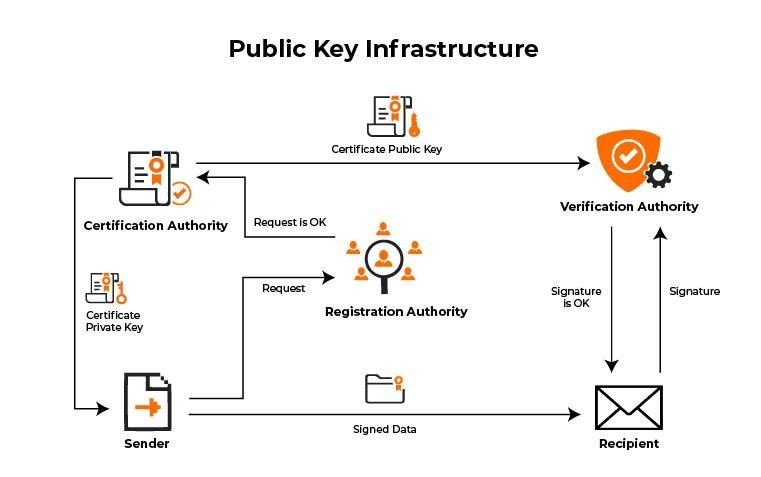
\includegraphics[scale=0.35]{Figures/pki.jpg}
    \caption{Public Key Infrastructure}
    \label{fig:pki}
\end{figure}

\noindent
Questo approccio consente una gestione scalabile delle chiavi.

\subsubsection*{Attacchi Quantum}

Gli schemi asimmetrici sono vulnerabili alla minaccia del quantum computer
Parlare degli algoritmi di Shor e ....



\subsection{Sicurezza}

Il \textbf{security level} è una misura della forza che una primitiva crittografica raggiunge rispetto ad attacchi.
Solitamente viene espresso come un numero di “bit di sicurezza”, dove $n$-bit di sicurezza significa che l'attaccante dovrebbe eseguire $2^n$ operazioni per romperlo.
\begin{itemize}
    \item Per i cifrari simmetrici il livello di sicurezza è pari alla dimensione del key-space. Equivale ad un attacco a forza bruta.
    \item La sicurezza dei cifrari simmetrici si basa su problemi matematici noti. Tuttavia, gli attacchi contro gli attuali sistemi a chiave pubblica sono sempre più veloci della ricerca a forza bruta dello spazio delle chiavi.
\end{itemize}

\noindent
Il NIST (National Institute of Standards and Technology) ha introdotto livelli di sicurezza, definiti in \textit{Tabella \ref{tab:security-levels}} per gli algoritmi di cifratura asimmetrica e post-quantistica come parte della sua iniziativa per standardizzare algoritmi che resistano anche ai computer quantistici.

% NIST Security Level Table
\begin{table}[ht]
    \centering
    \begin{tabular}{>{\centering\arraybackslash}m{3cm}p{10cm}}
        \toprule
        \textbf{Security Level} & \textbf{Descrizione} \\
        \midrule
        \textbf{Livello 1} & Sicurezza equivalente alla cifratura simmetrica con chiavi da 128 bit, come AES-128.\\
        \textbf{Livello 2} & Sicurezza equivalente ad attacchi contro SHA-256, con complessità circa pari a 128 bit. Leggermente più sicuro del livello 1. \\
        \textbf{Livello 3} & Sicurezza equivalente alla cifratura simmetrica con chiavi da 192 bit, come AES-192. \\
        \textbf{Livello 4} & Sicurezza equivalente ad attacchi contro SHA-384. Leggermente più sicuro del Livello 3. \\
        \textbf{Livello 5} & Sicurezza equivalente alla cifratura simmetrica con chiavi da 256 bit, come AES-256. \\
        \hline
    \end{tabular}
    \caption{Security Levels definiti dal NIST}
    \label{tab:security-levels}
\end{table}

\newpage
\section{Applicazioni}

Le reti, per loro natura, rappresentano un mezzo di comunicazione
intrinsecamente insicuro, soprattutto quando operano in modalità broadcast. In
questo contesto, la crittografia riveste un ruolo cruciale nel garantire la
sicurezza dei dati scambiati tra entità remote. I crittosistemi, ossia le
applicazioni crittografiche, integrano algoritmi di cifratura, autenticazione e
gestione delle chiavi per fare in modo che vengano rispettati i requisiti di sicurezza 
per le informazioni trasmesse.\\ 

\noindent
Il modello di riferimento per la comunicazione su Internet è il modello \textbf{TCP/IP}, il quale  suddivide il processo di trasmissione dei dati
in vari livelli, ciascuno con delle funzioni specifiche che non si sovrappongono con quelle degli altri livelli. Come mostrato in \textit{Figura \ref{fig:tcpip}},
è possibile applicare la sicurezza ai vari livelli della pila e di lato sono riportati i protocolli che vengono utilizzati. 

\begin{itemize}
    \item SSH (Secure Shell): Protegge l'accesso remoto e il trasferimento
    di file, fornendo autenticazione e cifratura.
    \item TLS (Transport Layer Security): permette di instaurare una
    connessione TCP sicura. Viene utilizzato per cifrare e autenticare i dati tra
    client e server.
    \item IPsec (Internet Protocol Security): Protegge i pacchetti IP
    scambiati tra due nodi, fornendo autenticazione, integrità e cifratura.
\end{itemize}

\begin{figure}[h!]
    \centering 
    \begin{tikzpicture} \matrix[matrix of nodes, nodes={anchor=center, minimum height=1cm}, 
        column 1/.style={nodes={draw, minimum width=5cm}}, 
        column 2/.style={nodes={align=left, text width=3cm}},
        row sep=-\pgflinewidth, column sep=5mm] (Layers) { 
            Application Layer & SSH, PGP \\
            Transport Layer & TLS        \\ 
            Network Layer & IPsec        \\ 
            Data Link Layer  & L2TP      \\ 
            Physical Layer & Hopping     \\ }; \foreach \i in {1,...,5}
    \draw[->] ([xshift=-5mm]Layers-\i-1.east)--(Layers-\i-2.west);
    \end{tikzpicture} 
    \caption{Stack TCP/IP} 
    \label{fig:tcp stack} 
    
\end{figure}

% MODELLO TCP/IP
\begin{comment}
    
    \begin{figure}[h!]
    \centering
    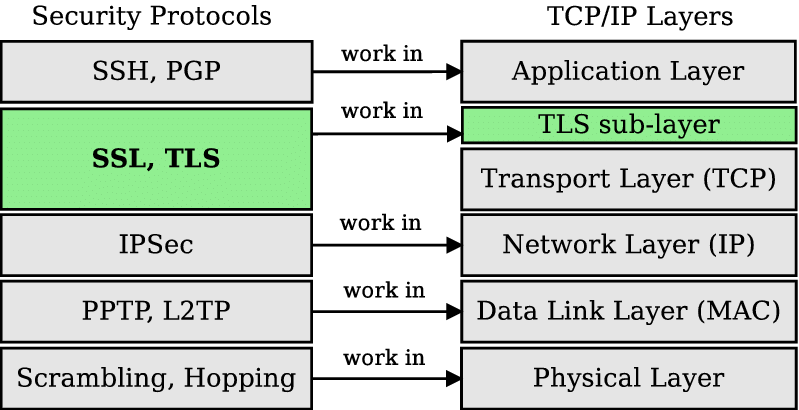
\includegraphics[scale=0.3]{Figures/security_tcp.png}
    \caption{Modello TCP/IP con Protocolli di Sicurezza}
    \label{fig:tcpip}
\end{figure}
\end{comment}

\noindent
Ogni protocollo avrà le proprie caratteristiche, tuttavia fare sicurezza a L3 dello stack TCP/IP offre un vantaggio significativo:
poiché tutti gli strati superiori dipendono da esso per la trasmissione dei dati,
non è necessario apportare modifiche ai singoli protocolli o applicazioni che
si basano su di esso. Questo consente di implementare soluzioni di sicurezza
centralizzate e trasparenti, senza dover intervenire su ciascun servizio o
applicazione a livello più alto.



\section{IPsec}

IPsec (Internet Protocol Security) è un insieme di protocolli standard, rappresentati in \textit{Figura \ref{fig:ipsec-suite}}, utilizzati
in modo tale da fornire meccanismi per l'autenticazione, la cifratura e l'integrità dei dati trasmessi tra due o più
dispositivi, proteggendo così le comunicazioni IP da intercettazioni e manomissioni.

\subsection{Architettura}

Come definito dall'\texttt{RFC 1825}, l'architettura di IPsec è composta dai seguenti componenti:

\begin{itemize}
    \item \textbf{AH (Authentication Header)}: si tratta di un protocollo di sicurezza che fornisce autenticazione e integrità dei dati,
    garantendo che i pacchetti non vengano modificati durante la trasmissione. Non offre cifratura, quindi i dati rimangono in chiaro. 
    \item \textbf{ESP (Encapsulating Security Payload)}: protocolo che fornisce cifratura per garantire la riservatezza dei dati,
    oltre a integrità e autenticazione opzionale. ESP è il protocollo più utilizzato
    per garantire sia sicurezza che riservatezza.
    
    \item \textbf{SA (Security Association)}: un insieme di parametri che definisce come i dati devono essere protetti durante la comunicazione tra due entità su una rete. Ogni SA contiene le informazioni necessarie per stabilire e mantenere una connessione sicura.
    \item \textbf{IKE (Internet Key Exchange)}: protocollo che consente di negoziare, autenticare e distribuire dinamicamente le chiavi crittografiche che vengono poi impiegate dai protocolli di sicurezza per proteggere le comunicazioni.
    \item \textbf{Algoritmi}: gli algoritmi crittografici e di hashing utilizzati per ottenere sicurezza.
\end{itemize}

\begin{figure}[!ht] 
    \centering 
    \scalebox{0.78}{
        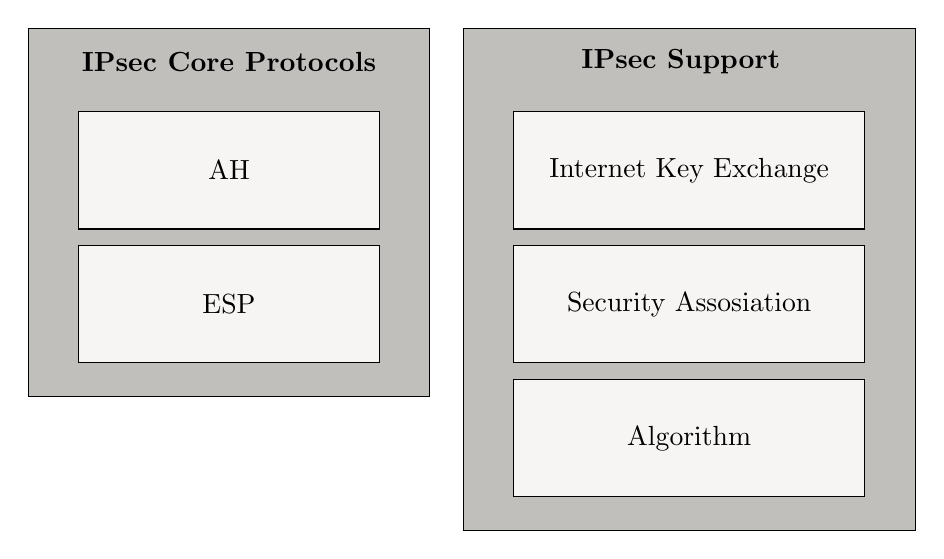
\begin{tikzpicture}[scale=0.85]
            \draw [ fill={rgb,255:red,192;green,191; blue,188} ] (5.5,13.25) rectangle (11.5,7.75); 
            \draw [ fill={rgb,255:red,246;green,245; blue,244} ] (6.25,10) rectangle node {ESP} (10.75,8.25); 
            \draw [ fill={rgb,255:red,192; green,191; blue,188} ] (12,13.25) rectangle (18.75,5.75); 
            \draw [ fill={rgb,255:red,246; green,245; blue,244} ] (6.25,12) rectangle node {AH} (10.75,10.25); 
            \node at (8.5,12.75) {\textbf{IPsec Core Protocols}}; 
            \node at (15.25,12.75) {\textbf{IPsec Support}}; 
            \draw [ fill={rgb,255:red,246; green,245; blue,244} ] (12.75,12) rectangle node { Internet Key Exchange} (18,10.25); 
            \draw [ fill={rgb,255:red,246; green,245; blue,244} ] (12.75,10) rectangle node { Security Assosiation} (18,8.25); 
            \draw [ fill={rgb,255:red,246; green,245; blue,244} ] (12.75,8) rectangle node { Algorithm} (18,6.25); 
        \end{tikzpicture}
    }
    \caption{IPsec Protolocol Suite}
    \label{fig:ipsec-suite} 
\end{figure}
    

\subsection{Security Association}

IP è un protocollo \textit{stateless}, ovvero non mantiene informazioni o stato relativo alle connessioni o ai pacchetti che gestisce.
Tuttavia affinchè IPsec possa garantire la sicurezza è necessario che mantenga il contesto di ogni connessione, le principali motivazioni sono:
\begin{itemize}
    \item \textit{Replay Protection}: per evitare attacchi di tipo reply, IPsec tiene  traccia
    dei numeri di sequenza dei pacchetti, un'inforamzione di stato che va mantenuta per ogni connessioni
    e che IP non fa nativamente.
    \item \textit{Connessioni Multiple}: in uno scenario di rete complesso, un singolo dispositivo potrebbe avere più connessioni sicure in corso simultaneamenamente, ognuna
    delle quali ha i propri parametri di sicurezza. IPsec deve tenere traccia di queste informazioni per sapere come trattare i pacchetti in entrata e uscita in base alla connessione a cui appartengono.
    \item \textit{Protezione}: i protocolli di sicurezza AH e ESP richiedono di conoscere le chiavi crittografiche corrette e gli algoritmi utilizzati per cifrare e decifrare i pacchetti.
\end{itemize}

\noindent 
IP diventa in grado di mantenere un'insieme di informazioni di stato grazie al concetto di \textit{Security Association} (SA).
Più precisamente si tratta di un'insieme di parametri che servono per associare a ciascun canale uno stato condiviso tra le entità coinvolte nello comunicazione,
tra questi abbiamo:

\begin{itemize}
    \item \textit{Security Parameter Index} (SPI): un'identificatore della SA.
    \item \textit{Destination Address}: serve all'host per determinare quale SA utilizzare. 
    \item \textit{Lifetime}: il tempo di vita della SA, si obbliga a refresh periodici.
    \item \textit{Protocol Identifier}: determina il tipo di protezione da applicare ai pacchetti, dunque anche chiavi e algoritmi associati.
    \item Altri parametri opzionali, per una lista completa fare riferimento all'RFC.
\end{itemize}

\noindent
La SA è caratterizzata dall'essere un canale \textit{simplex}, dunque al fine di stabilire un canale di comunicazione bidirezionale IPsec tra due entità occorrono due SA unidirezionali di verso opposto.
La \textit{Figura \ref{fig:sa_bidirezionale}} mostra il tunnerl virtuale in esecuzione tra i due host.
%aggiungere al lato di un host la configurazione dell'SA
\begin{figure}[h!]
    \centering
    \begin{tikzpicture}
        \node (router_a) [router] {Host A};
        \node (router_b) [router, right of=router_a, xshift=5cm] {Host B};
        \draw (router_a) ++(0.8,0) ellipse (0.2cm and 0.2cm);
        \draw [-] (0.8,0.2) -- (5.25,0.2) node[midway, above]{\inlinecode{SA\_AB}};
        \draw [-] (0.8,-0.2) -- (5.25,-0.2) node[midway, below]{\inlinecode{SA\_BA}};
        \draw (router_b) ++(-0.8,0) ellipse (0.2cm and 0.2cm);   
    \end{tikzpicture}
    \vspace{0.4cm}
    \caption{Security Association bidirezionali}
    \label{fig:sa_bidirezionale}
\end{figure}

\noindent

\subsection{Negoziazione SA}

In un contesto come quello delle reti potremmo avere che lo stesso nodo ha connessini IPsec multiple, 
le SA consentono di distinguere e identificare in modo univoco la configurazioni di sicurezza da applicare alla comunicazione.\\
Tuttavia queste SA come si configurano?.
IPsec prevede tecniche di negoziazione delle SA di tipo:

\begin{itemize}
    \item \textit{Manuale}: occorre configurire manualmente le chiavi e le
    impostazioni di sicurezza per ciascun dispositivo o punto finale di
    comunicazione.
    \item \textit{Automatico}: si utilizzanoprotocolli per stabilire
    automaticamente le chiavi di crittografia e le politiche di sicurezza senza
    intervento umano diretto.
\end{itemize}
\noindent
L'utilizzo di tecniche di negoziazione automatica offre un approccio sicuro, flessibile e scalabile alla gestione delle Security Association, un esempio di questo è IKE.
Andiamo a vedere nel dettaglio IKE nella prossima sezione.

\newpage
\section{IKE}
Questo protocollo definisce una serie di scambi, mostrati in \textit{Figura \ref{fig:ike_exchange}}, al termine del quale i due peer avranno negioziati i parametri di sicurezza e le chiavi crittografiche per una SA.

\begin{figure}[htbp]
    \centering
    \begin{tikzpicture}[node distance=1.5cm]
        % Initiator and Responder
        \node (entity1) [draw=red, rectangle] {Initiator (\textit{i})};
        \node (entity2) [draw=blue, rectangle, right=of entity1, xshift=3cm] {Responder (\textit{r})};
        \draw (entity1) -- ++(0,-6.7) coordinate (vertical1);
        \draw (entity2) -- ++(0,-6.7);
        % IKE_INIT_SA
        \draw[-stealth] (entity1) ++(0,-1) -- (entity2 |-,-1) node[midway, above, text=red, font=\footnotesize] {Request};
        \draw[stealth-] (entity1) ++(0,-2) -- (entity2 |-,-2) node[midway, above, text=blue, font=\footnotesize] {Response};
        % IKE_AUTH
        \draw[-stealth] (entity1) ++(0,-3.5) -- (entity2 |-,-3.5) node[midway, above, text=red, font=\footnotesize] {Request};
        \draw[stealth-] (entity1) ++(0,-4.5) -- (entity2 |-,-4.5) node[midway, above, text=blue, font=\footnotesize] {Response};
        % CHILD_SA 
        \node at (-1.7,-6) {\inlinecode{CHILD\_SA}};
        \node at (-2,-1.5) {\inlinecode{IKE\_SA\_INIT}};
        \node at (-1.7,-4) {\inlinecode{IKE\_AUTH}};
        \draw (entity1) ++(0.2,-6) ellipse (0.2cm and 0.2cm);
        \draw [-] (0.2,-6.2) -- (6.65,-6.2);
        \draw [-] (0.2,-5.8) -- (6.65,-5.8) node[midway, above, font=\footnotesize]{$SK_d, N_i, N_r$};
        \draw (entity2) ++(-0.2,-6) ellipse (0.2cm and 0.2cm);
        % Key for encryption and authtenticatoin
        \drawkey{-1, -2.3}{red}{$SK_{ei}$};
        \drawkey{-1.8, -2.3}{red}{$SK_{ai}$};
        \drawkey{8, -2.3}{blue}{$SK_{ar}$};
        \drawkey{8.8, -2.3}{blue}{$SK_{er}$};
        % Group
        \drawcurlybrace{0,-1}{0, -2}{};
        \drawcurlybrace{0,-3.5}{0, -4.5}{};
    \end{tikzpicture}
    \caption{Fasi di Negoziazione del Protocollo IKEv2}
    \label{fig:ike_exchange}
\end{figure}


\subsection{\textbf{IKE\_SA\_INIT}}

Lo scopo di questa prima fase è quello di creare una \textbf{IKE SA}, che consenta di rendere sicure i successivi scambi di dati al fine di realizzare una \textbf{IPsec SA}.
Dunque funge da apripista al fine di stabilire quelli che sono i parametri di sicurezza al fine di avere una comunicazione sicura. Per questo motivo in questo scambio i peer 
si scambiano le seguenti informazioni:

\begin{table}[htbp]
    \centering
    \caption{Tabella dei parametri e delle descrizioni}
    \begin{tabular}{ll}
        \toprule
        \textbf{Parametro} & \textbf{Descrizione} \\
        \midrule
        \textit{SA} & Security Association, vengono negoziati i parametri per la SA\\
        \textit{KE} & Key Exchange, e nel caso classico è l'esponente DH \\
        \textit{N} & Nonce \\
    \bottomrule
    \end{tabular}
\end{table}

\noindent
Al termine di questo scambio i due peer ottengono il \textit{DH Shared Secret} (indicato con $g^{ir}$), il quale insisme ai nonce, consentirà di ottenere 
quelli che sono i parametri di sicurezza della $IKE SA$ al fine di instauare un canale sicuro, per approfondimenti in \href{AppendixA}{appendice}.

% Tabella che riporta le varie funzioni delle chiavi

\subsection{IKE\_AUTH}

Il risultato della fase precedente è un canale sicuro su cui comunicare, in quanto è cifrato e utenticato. Si questo hanno luogo gli scambi per instaurare la IPsec SA.
In questa fase i nodi si autenticano mutuamente:

\begin{table}[htbp]
    \centering
    \caption{Tabella dei parametri e delle descrizioni}
    \begin{tabular}{ll}
        \toprule
        \textbf{Parametro} & \textbf{Descrizione} \\
        \midrule
        \textit{AUTH} & Payload che deve essere firmato affinchè ci sia autenticazione \\
        \textit{CERT} & Si allega il certificato digitale per la chiave pubblica \\
        \textit{CERTQ} & Si fa richiesta al peer di fornire il certificato \\
    \bottomrule
    \end{tabular}
\end{table}

Tutto il contenuto appena descritto è protetto mediante le chiavi segrete di quella direzione. Ciò è indicato mediante la notazione $SK\{...\}$
La modalità di autenticazione può essere: PSK, EAP oppure mediante chiave pubblica.

\subsection{CHILD\_SA}


\section{Problemi}

IKEv2 utilizza come porotocollo a livello trasporto UDP per per inoltrare i propri messaggi. La maggior parte dei messaggi che i peer si scambiano hanno dimensioni relativamente piccole e
quindi che non eccedono l'\textbf{MTU} di un pacchetto IP, tuttavia abbiamo degli scambi che richiedono un trasferimento di dati abbastanza grandi.

Per esempio nel caso di autenticazione tramite pubkey nella fase di \inlinecode{IKE\_AUTH} è necessario trasferire il proprio certificato che in base allo schema di firma utilizzato
può arrivare anche a diversi Kbyte di dimensione. In questi casi si verifica la frammentazione a livello IP.

%Immagine frammentazione

\begin{figure}[htbp]
    \centering
    \begin{tikzpicture}[node distance=2cm,>=Latex]
        % Nodi
        \node (initiator) [client] {Initiator};
        \node (device) [router, right=of initiator] {Device};
        \node (responder) [client, right=of device] {Responder};
        \node (message) [messageclosed, fill=orange!40, minimum size=0.6cm] at (1.9,0.5) {};
        \node (message2) [messageclosed, fill=gray!40, minimum size=0.6cm] at (1.2,0.5) {};
        \node (drop) [messageclosed, fill=gray!40, minimum size=0.6cm, , font=\small, text=red] at (3,1) {};
        \node (message3) [messageclosed, fill=orange!40, minimum size=0.6cm, , font=\small, text=red] at (4.5,0.5) {};

        \draw[-] (initiator.east) -- (device.west);
        \draw[-] (device.east) -- (responder.west);

    \end{tikzpicture}
    \vspace*{1cm}
    \caption{Drop Pacchetti}
    \label{fig:cgnatdrop}
\end{figure}

Diversi test hanno mostrato che nel caso in cui i peer si trovino in presenza di CGNAT potrebbero non istausarsi le SA. Questo è dovuto al fatto che i device degli ISP non
consentono ai frammenti IP di passare attravers di loro, ovvero scartano i pacchetti e di conseguenza bloccano le comunicazioni IKE.
Questo è riportato schematicamente in Fig. \ref{fig:cgnatdrop}.
Questo drop dei pacchetti avviene perchè esistono numerosi vettori di attacco che fanno affidamento sulla frammentazione IP, per questo motivo gli ISP operano un filtro su questa tipologia di pacchetti.
Ance se in teoria uno dei requisiti del CGNAT definito dagli RFC è proprio consentire la frammentazione.

Per risolvere questa problematica e dunque consentire il passaggio dei messaggi attraverso i dispositivi di rete che non consentono il passaggio degli IP fragment attraverso 
di loro nell' RFC 7283 viene introdotta la IKEv2 \textit{Message Fragmentation}. In cui la frammentazione dei messaggi è gestita direttamente da parte di chi implementa IKEv2

\subsection{\inlinecode{IKE\_INTERMEDIATE}}

Per evitare che nel trasferimento di grandi dati ciò avvenga viene introdotto uno scambio aggiuntivo. Questo scambio è introdotto per quei casi in cui la dimensione dei dati
da trasferire ecceda la dimensione massima che causerebbe la frammentazione IP. Questo scambio va fatto dopo la \inlinecode{IKE\_INIT\_SA} e prima della \inlinecode{IKE\_AUTH} in questo
modo è sia autenticato che cifrato tramite le chiavi negoziate dal primo scambio.

\begin{figure}[htbp]
    \centering
    \begin{tikzpicture}[node distance=1.5cm]
        % Initiator and Responder
        \node (entity1) [draw=red, rectangle] {Initiator (\textit{i})};
        \node (entity2) [draw=blue, rectangle, right=of entity1, xshift=3cm] {Responder (\textit{r})};
        \draw (entity1) -- ++(0,-4.5) coordinate (vertical1);
        \draw (entity2) -- ++(0,-4.5);
        % IKE_AUTH
        \draw[stealth-stealth] (entity1) ++(0,-1.5) -- (entity2 |-,-1.5) node[midway, above] {\inlinecode{IKE\_SA\_INIT}};
        \draw[stealth-stealth] (entity1) ++(0,-2.5) -- (entity2 |-,-2.5) node[midway, above] {[\inlinecode{IKE\_INTERMEDIATE}]};
        \draw[stealth-stealth] (entity1) ++(0,-3.5) -- (entity2 |-,-3.5) node[midway, above] {\inlinecode{IKE\_AUTH}};
    \end{tikzpicture}
    \caption{Scambio nuovo}
    \label{fig:ikeintermediate}
\end{figure}

Questo scambio è posizionato qui in quanto nella \inlinecode{IKE\_SA\_INIT} per motivi di sicurezza non è possibile applicare la frammentazione.
Di solito i messaggi sono piccoli abbastanza da non causare la frammentazione IP, tuttavia questo potrebbe cambiare se si utilizzano scambi di chiave QC-resistant; in quanto
hanno chiavi pubbliche larghe e che quindi causerebbero frammentazione IP.

Per questo viene aggiunto questo scambio che viene utilizzato per trasferire grandi quantità di dati.

L'utilizzo principale di questo scambio è quello di trasferire le chiavi pubbliche QC-resistant, tuttavia in generale può essere utilizzzato per trasferire qualsiasi tipologia di dato.
Quindi il principale utilizzo è quello di fare un \textbf{enforcing} delle chiavi negoziate tramite DH al fine di renderle QC-resistant. Infatti se durante questo scambio si scambiano 
altre chiavi allora le coppie $\{SK_{a[i/r]}, SK_{e[i/r]}\}$ vengono aggiornate.

Permette di realizzare Multiple Key Exchange
Gli scambi di chiave aggiuntivi vengono aggiunti alla proposal tramite \inlinecode{PQ\_KEM\_1}



Lo scambio \inlinecode{IKE\_FOLLOWUP\_KE} è introdotto specificatamente per trasferire dati sulla chiavi addizionali da realizzare in una CHILD SA.
In questo caso le chiavi aggiuntive vengono utilizzate per aggiornare il KEYMAT



\begin{itemize}
    \item flag \inlinecode{IKE\_FRAGMENTATION\_SUPPORT}: il peer dice di supportare la frammentazione IKEv2, affinchè venga utilizzata entrambi i peer devono supportarla.
    \item flag \inlinecode{INTERMEDIATE\_EXCHANGE\_SUPPORT}: il peer dice di supportare gli scambi intermedi
\end{itemize}

Una volta terminati gli scambi, per proteggere lo scambio \inlinecode{IKE\_AUTH} e gli scambi successivi vengno utilizzata le ultime chiavi calcolate
Dato che i dati trasferiti in questi scambi aggiuntivi vanno autenticati si aggiungono all'\inlinecode{AUTH} payload che poi andrà 



Il supporto per lo scambio aggiuntivo viene comunicato aggiungendo all'interno
dell \inlinecode{IKE\_SA\_INIT} il flag \inlinecode{IKE\_INT\_SUP} (che sta per
Intermediate Exchange Support).
Se anche il responder lo supporta lo includerà nel messaggio di risposta dello
scambio.




Considerazioni, L'IKE fragmentation viene introdotta a causa del NAT tuttavia nel nostro caso di satelliti non ha senso utilizzarla in quanto non credo che si utilizzi
il NAT soprattutto perchè introduce ritardi dovuti alla traduzione degli indirizzi



\section{Post-Quantum}

Un solo KEM con Kyber L1 usando come suite AES\_GCM has vabene come certificato dilithium L1

Nel KEM quanti cifrano?

Cioè l'initiator manda il certificato e poi il responder cifra 
